\documentclass[10pt]{article}

\usepackage[left=0.8in,right=0.8in,top=0.15in,bottom=0.8in]{geometry}
\usepackage{xcolor}
\usepackage{hyperref}
\usepackage{graphicx}
\usepackage{float}

\hypersetup{colorlinks=true,linkcolor=blue,urlcolor=blue}
\urlstyle{rm}
\usepackage{url}
\usepackage{amsmath}



\title{CAI 4104: Machine Learning Engineering\\
	\large Project Report:  {\textcolor{purple}{Object Classification}}} %% TODO: replace with the title of your project
	
	
	
%% TODO: your name and email go here (all members of the group)
%% Comment out as needed and designate a point of contact
%% Add / remove names as necessary
\author{
        Khang Tran \\
        trankhang@ufl.edu\\
        \and
        Nicolas Slenko \\
        nslenko@ufl.edu\\
        \and
        Colin Wishart \\
        c.wishart@ufl.edu\\
        \and
        Christopher Dowdy \\
        cdowdy@ufl.edu\\
        \and
        Mauro Chavez Vega \\
        maurochavezvega@ufl.edu\\
}


% set the date to today
\date{\today}


\begin{document} % start document tag

\maketitle



%%% Remember: writing counts! (try to be clear and concise.)
%%% Make sure to cite your sources and references (use refs.bib and \cite{} or \footnote{} for URLs).
%%%



%% TODO: write an introduction to make the report self-contained
%% Must address:
%% - What is the project about and what is notable about the approach and results?
%%
\section{Introduction}

% TODO:
Given a dataset containing 128 x 128 RGB PNG images containing one of 12 different objects: backpack, book, calculator, chair, clock, desk, keychain, laptop, paper, pen, phone, water bottle. The
goal of this project is to correctly classify images into one of the 12 classes mentioned above. The dataset is split into 70\% training, 15\% validation and 15\% testing. We will use a 
convolutional neural network (CNN) to classify the images. The CNN will consist of several convolutional layers, followed by max pooling layers, and finally fully connected layers. 
We will use the Adam optimizer and categorical cross-entropy loss function to train the model. The model will be evaluated using accuracy and per class accuracy.

\begin{figure}[H]
    \centering
    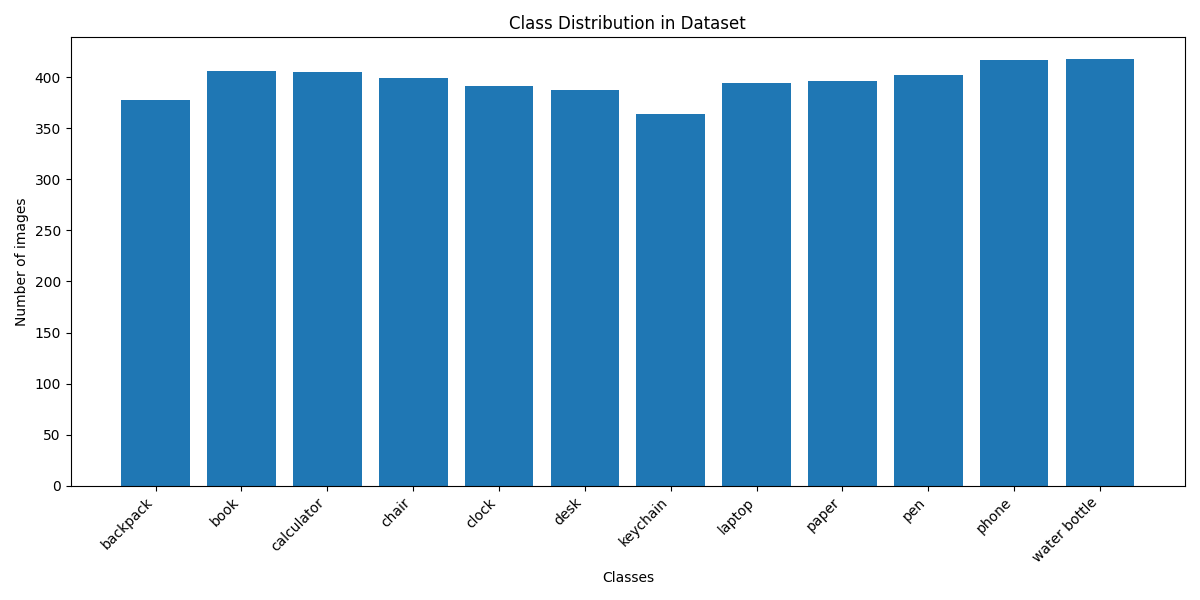
\includegraphics[width=0.9\textwidth]{figures/class_distribution.png}
    \caption{Distribution of images across the 12 object classes in the dataset. The dataset is relatively balanced, with each class containing between 360-420 images.}
    \label{fig:class_distribution}
\end{figure}

%% TODO: write about your approach / ML pipeline
%% Must contain:
%% - How you are trying to solve this problem
%% - How did you process the data?
%% - What is the task and approach (ML techniques)?
%%
\section{Approach}

\subsection{Data Preprocessing}

Our data preprocessing pipeline consists of several key steps to prepare the images for training:

\begin{itemize}
    \item \textbf{Image Resizing:} Although it is assumed that all the images are 128x128 pixels, we still resized all the images to 128x128 pixels to ensure uniformity.
    and that the expected batch size match the input size of the model.
    
    \item \textbf{Normalization:} The input were first applied with transform.ToTensor which would have perfomed scaling on the pixel values from the range of [0, 255] to [0, 1]. 
    All images were then normalized using mean = [0.5, 0.5, 0.5] and standard deviation = [0.5, 0.5, 0.5] for each color channel to center the data around 0 and remap it to a range of 
    [-1, 1] and ensure consistent scale.
    
    \item \textbf{Data Splitting:} We divided the dataset into three subsets:
    \begin{itemize}
        \item Training set: 70\% of the data
        \item Validation set: 15\% of the data
        \item Test set: 15\% of the data
    \end{itemize}
    We decided on that this data splitting ratio since that is what was recommended for small dataset (under 100k examples) such as the dataset we are using to train this project model.
\end{itemize}

\subsection{Model Architecture}

Since the problem at hand is clearly a multi-class classification problem, we decided to use a convolutional neural network (CNN) architecture which generally performs well on computer vision tasks
or task related to image data. We implemented a custom CNN architecture with the following layers:

\begin{itemize}
    \item \textbf{Data Augmentation:} Since the given dataset only consists of 4757 images, which is relatively small, we applied data augmentation to just the
    training set to artificially increase training diversity. Furthermore, this also act as a regularization technique to prevent overfitting which we later
    encountered during training. The data augmentation techniques we used include:
    \begin{itemize}
        \item Random horizontal flips to 50 percent of the images
        \item Random vertical flips to 50 percent of the images
        \item Random rotations (up to 15 degrees) to 50 percent of the images
    \end{itemize}
    These techniques should help the model generalize better to unseen data as the objects in real life might appear in different orientations.

    \item \textbf{Convolutional Layers:} Five convolutional blocks, each containing:
    \begin{itemize}
        \item A convolutional layer with increasing filter depths (starting from base filters and increasing)
        \item Batch normalization for further improved training stability
        \item ReLU activation function
        \item Max pooling layer
        \item Dropout for regularization
    \end{itemize}
    We decided to go with a stretch pants like approach where we made our layers wider and then use dropout in between them.

    \item \textbf{Fully Connected Layers:} Two fully connected layers:
    \begin{itemize}
        \item A flatten layer that reshape the 512x4x4 feature map into a 8192-dimensional vector
        \item A hidden layer with dropout regularization of 0.5 to prevent overfitting
        \item An output layer with 12 neurons (one for each class)
    \end{itemize}

    \item \textbf{Loss Function:} Cross-entropy loss since it is a classification problem with label smoothing of 0.1, which helps prevent the model from becoming overconfident and reduce overfitting
    
    \item \textbf{Optimizer:} Adam optimizer with a learning rate of 0.0005 and weight decay (L2 regularization) of 0.0005
\end{itemize}

This architecture was designed to extracting higher-level features through the deep convolutional layers for good performance while still preventing overfitting through the use of regularization techniques.

\subsection{Training Strategy}

\begin{itemize}
    \item \textbf{Learning Rate Scheduling:} We implemented a ReduceLROnPlateau scheduler that reduces the learning rate by a factor of 0.5 when validation accuracy plateaus for 4 consecutive epochs
    
    \item \textbf{Early Stopping:} Training terminates if validation loss doesn't improve for 10 consecutive epochs, preventing overfitting
    
    \item \textbf{Model Checkpointing:} We saved both an early-stopped model and the final model after training completion for faster evaluation and testing
\end{itemize}

\subsection{Training Process Visualization}

\begin{figure}[H]
    \centering
    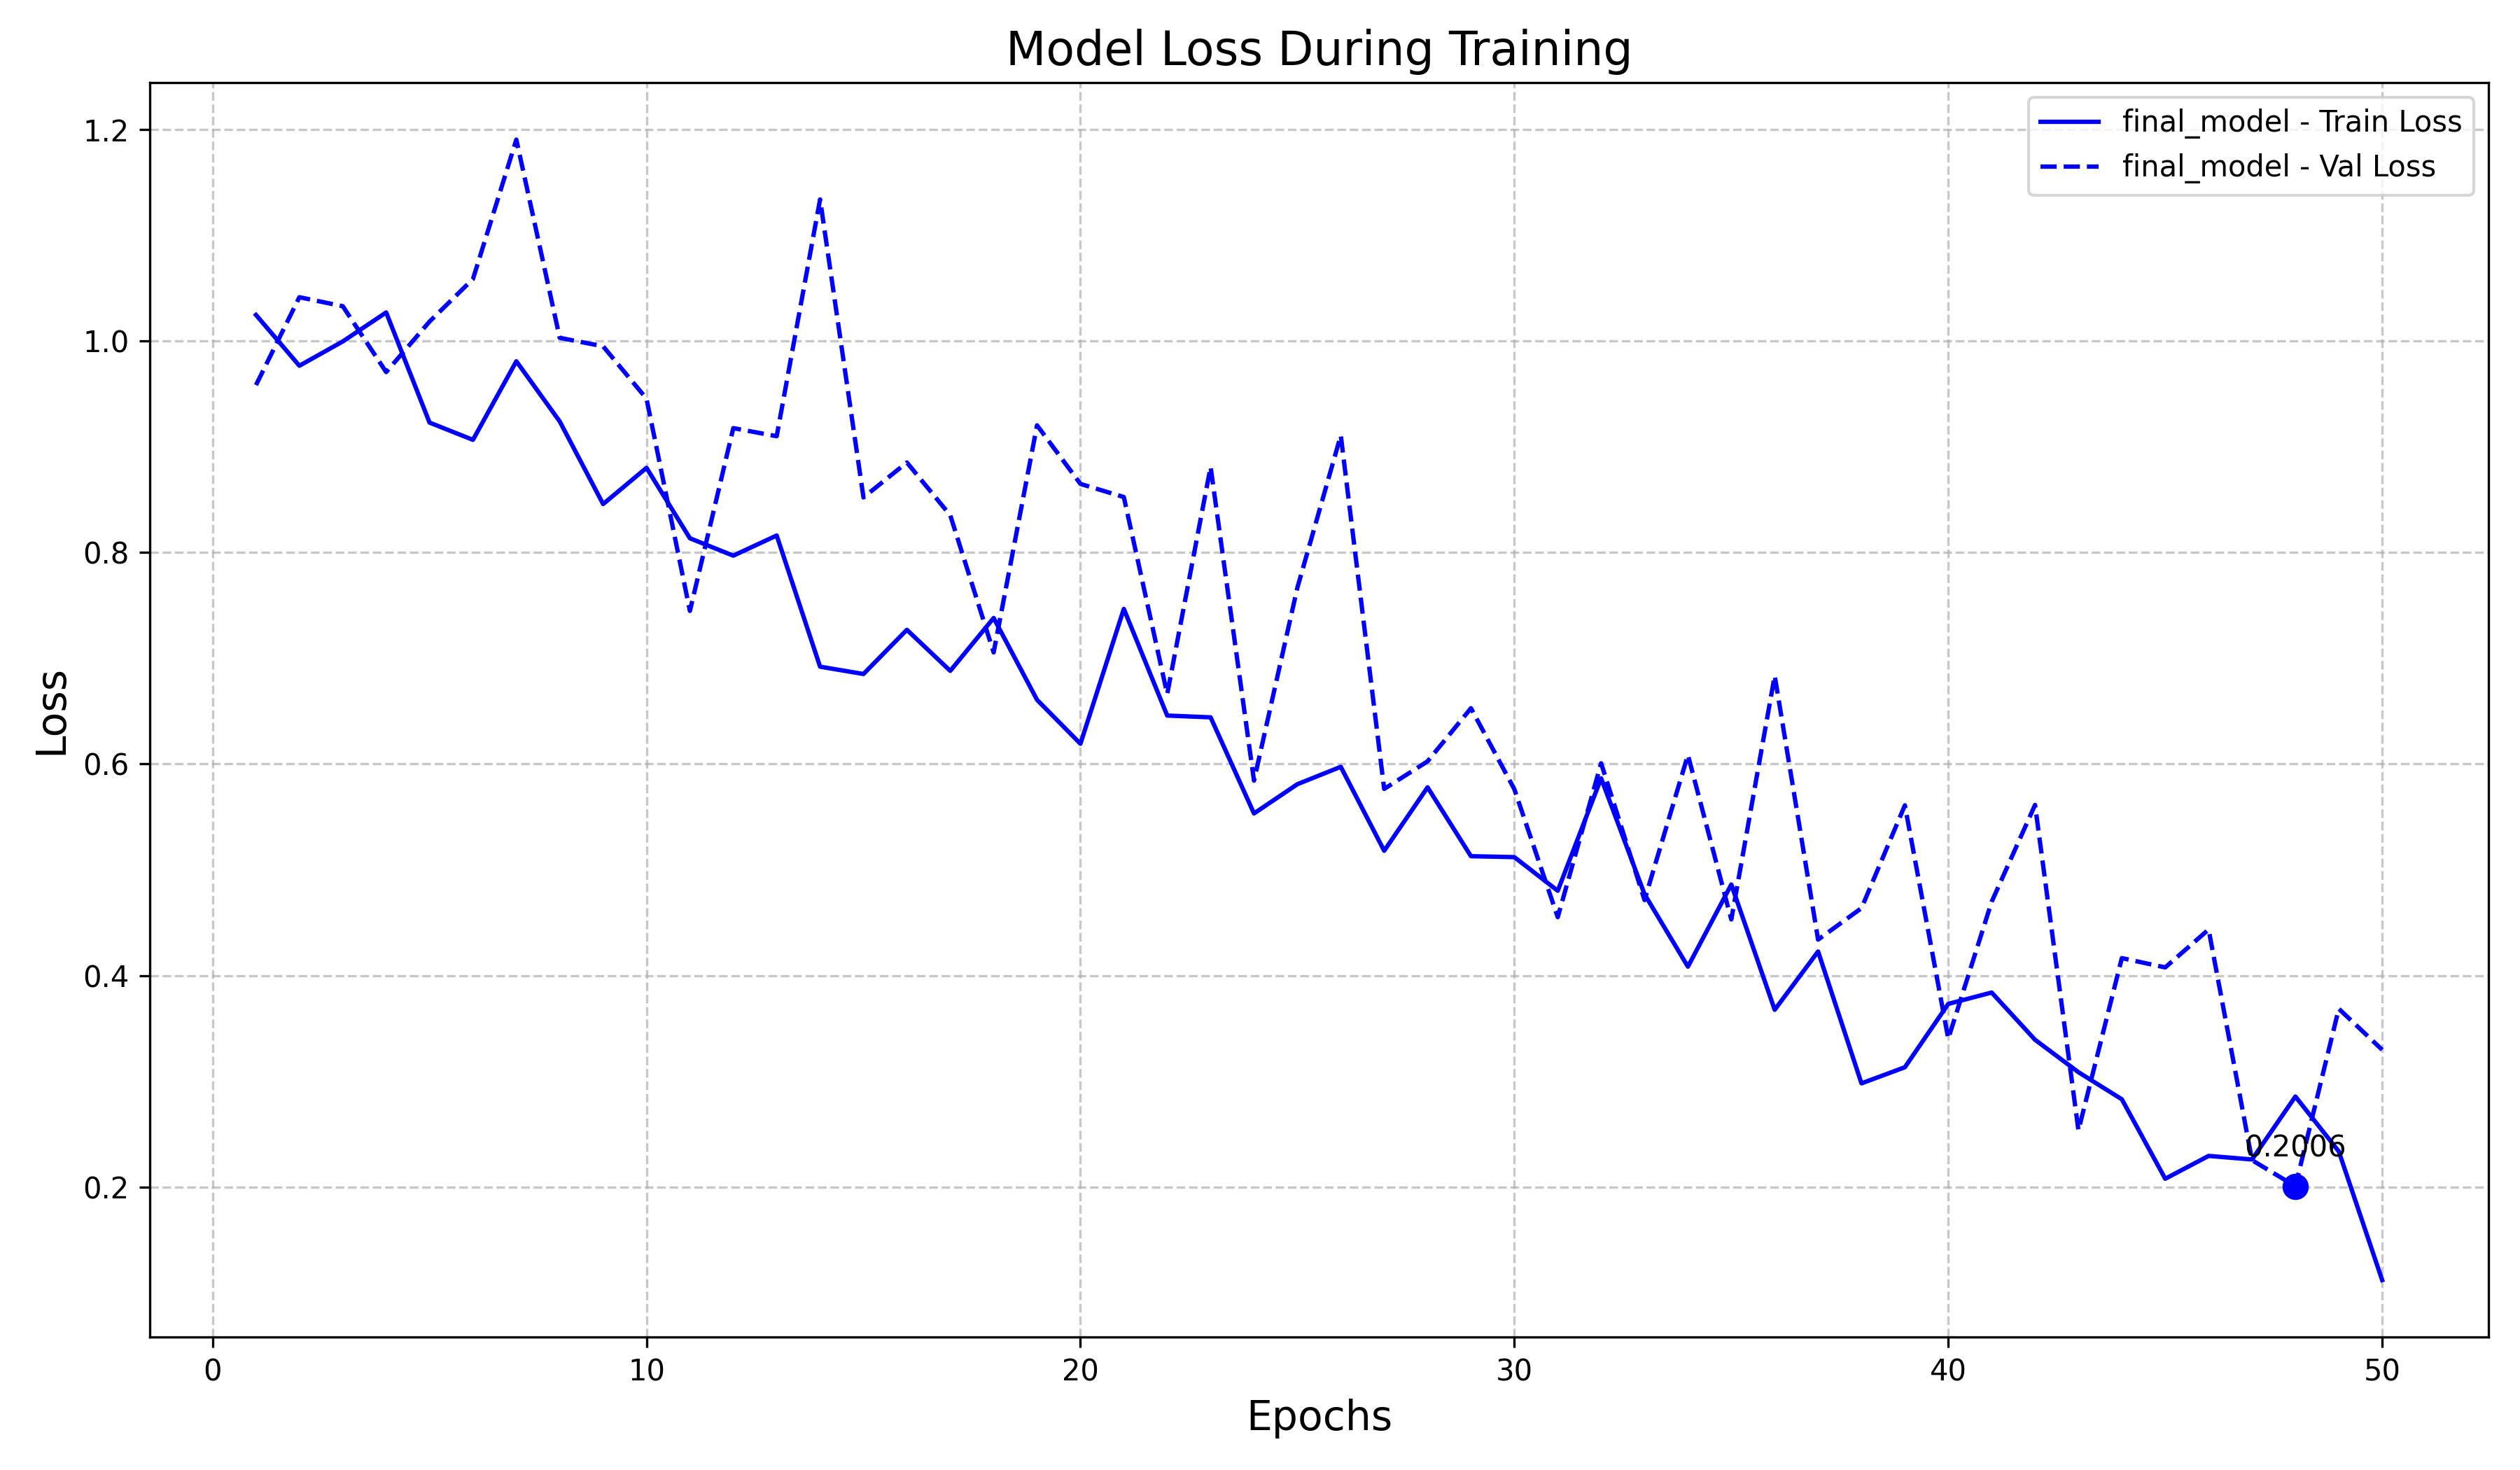
\includegraphics[width=0.9\textwidth]{figures/loss_curves.png}
    \caption{Model loss during training. The training loss (solid line) and validation loss (dashed line) both decrease over time, indicating successful learning.}
    \label{fig:model_loss}
\end{figure}

\begin{figure}[H]
    \centering
    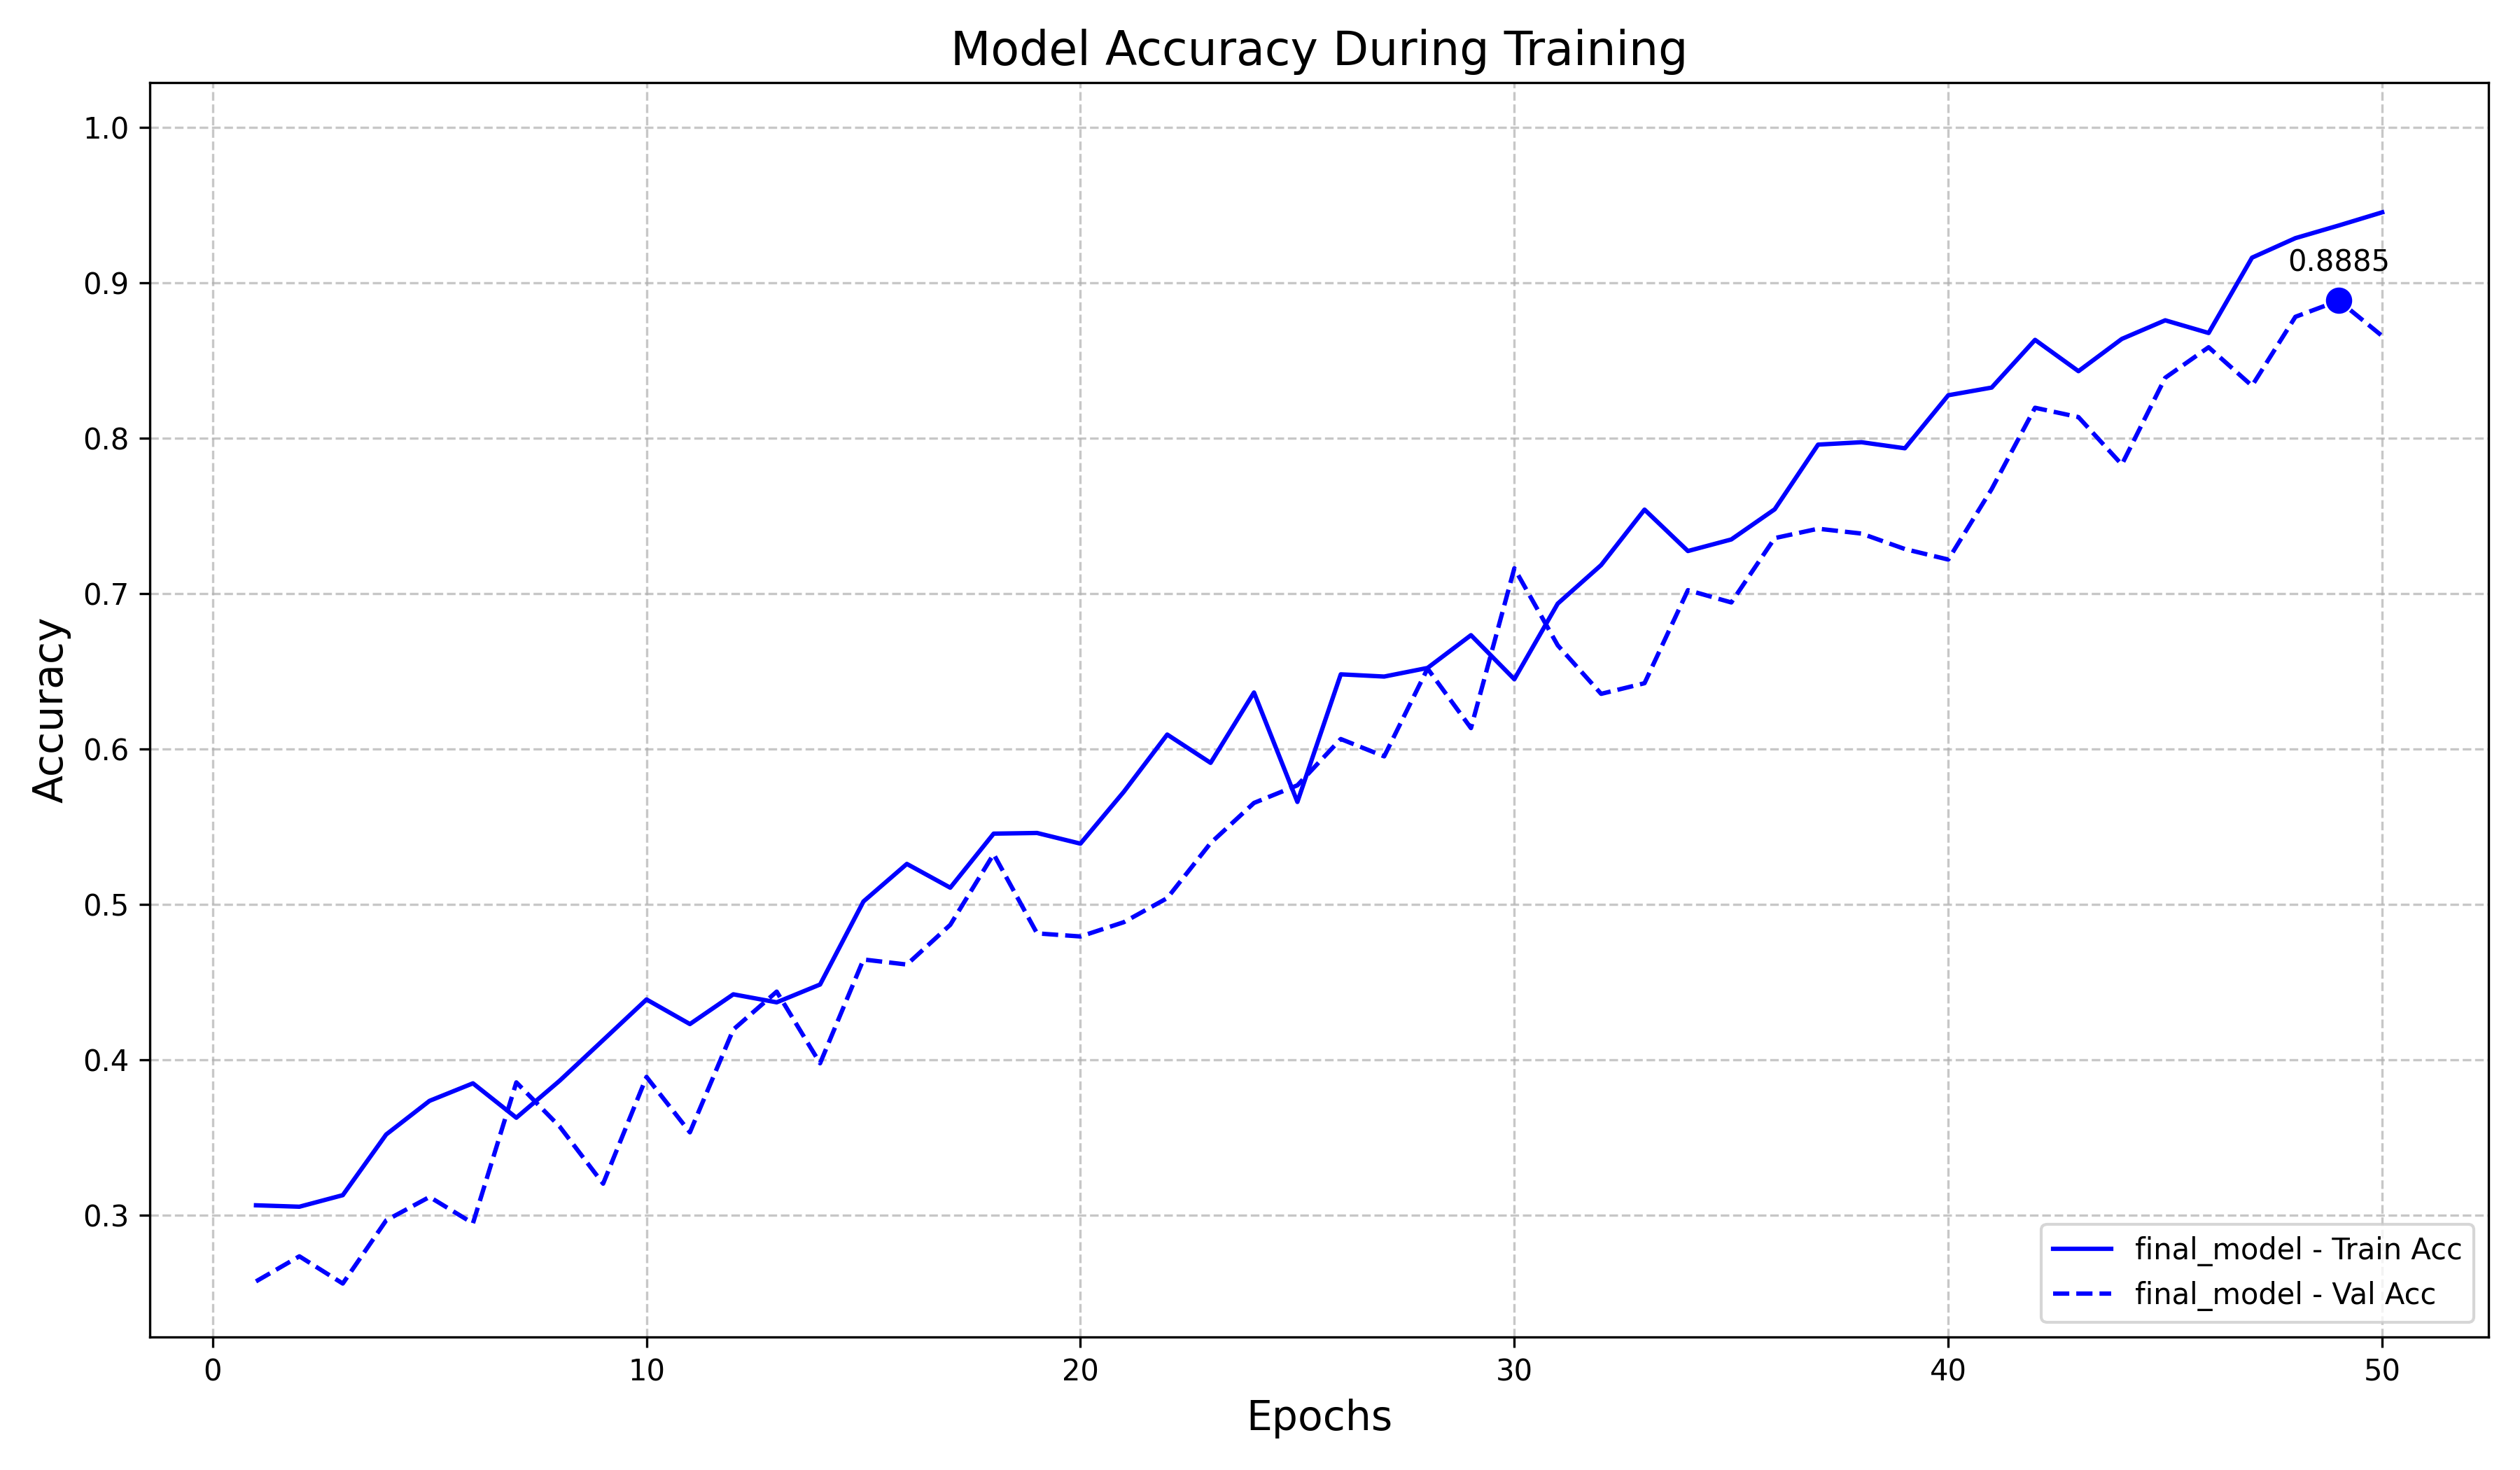
\includegraphics[width=0.9\textwidth]{figures/accuracy_curves.png}
    \caption{Model accuracy during training. The training accuracy (solid line) and validation accuracy (dashed line) both increase over time, with final validation accuracy reaching approximately 88.85\%. Note that this validation accuracy differs from the 78.43\% test accuracy reported in Table \ref{tab:test_summary}, as they are evaluated on different datasets.}
    \label{fig:model_accuracy}
\end{figure}




%% TODO: write about your evaluation methodology
%% Must contain:
%% - What are the metrics?
%% - What are the baselines?
%% - How did you split the data?
%%
\section{Evaluation Methodology}

\begin{itemize}
    \item \textbf{Metrics:} Since this is a multi-class classification problem, we used the following metrics to evaluate our model:
    \begin{itemize}
        \item Accuracy: To measure the overall performance of the model
        \item Per-class accuracy: The accuracy for each class to evaluate the model's performance on each class
    \end{itemize}

    \item \textbf{Baselines:} We compared our model's performance by evaluating the metrics mentioned above against a random guessing model as a baseline.

    \item \textbf{Data Split:} As mentioned in our preprocessing section, we used a 70\%-15\%-15\% train-val-test split on our dataset.
    
    \item \textbf{Hyperparameter Tuning:} The hyperparameters that were tuned in our model include:
    \begin{itemize}
        \item Different learning rates (0.0001, 0.0005, 0.001)
        \item Different batch sizes (32, 64, 128) with 64 being the most optimal for learning speed and computation time
        \item Different dropout rates in both convolutional (0.1) and fully connected (0.5) layers
        \item Different weight decay values for regularization (0.0001, 0.0005, 0.001)
        \item Different numbers of convolutional blocks (3, 5, 7) with 5 being the most optimal for learning speed and computation time
    \end{itemize}
    
    \item \textbf{Model Selection:} The final model was selected based on the best accuracy and per class accuracy on the test set. Additionally, we also considered the model's performance on the 
    validation set to ensure that overfitting was at an acceptable level.
\end{itemize}





%% TODO: write about your results/findings
%% Must contain:
%% - results comparing your approach to baseline according to metrics
%%
%% You can present this information in whatever way you want but consider tables and (or) figures.
%%
\section{Results}

\subsection{Test-Set Composition}

The test set contains a total of 714 images distributed among the 12 classes as follows:

\begin{table}[h!]
    \centering
    \caption{Test-set image counts by class}
    \label{tab:test_counts}
    \begin{tabular}{|l|r|}
        \hline
        \textbf{Class}       & \textbf{Image Count} \\ \hline
        Backpack             & 68                   \\
        Book                 & 53                   \\
        Calculator           & 65                   \\
        Chair                & 60                   \\
        Clock                & 57                   \\
        Desk                 & 55                   \\
        Keychain             & 59                   \\
        Laptop               & 60                   \\
        Paper                & 57                   \\
        Pen                  & 47                   \\
        Phone                & 73                   \\
        Water Bottle         & 60                   \\ \hline
        \textbf{Total}       & \textbf{714}         \\ \hline
    \end{tabular}
\end{table}

\subsection{Accuracy Comparison}
\begin{table}[h!]
    \centering
    \caption{Per-class and overall performance: CNN vs.\ random baseline}
    \label{tab:test_summary}
        \begin{tabular}{|l|c|c|c|}
        \hline
        \textbf{Class}       & \textbf{CNN Accuracy (\%)} & \textbf{Random Baseline (\%)} & \textbf{Improvement (\%)} \\ \hline
        Backpack             & 76.47                      & 7.35                           & 69.12                     \\
        Book                 & 77.36                      & 7.55                           & 69.81                     \\
        Calculator           & 87.69                      & 9.23                           & 78.46                     \\
        Chair                & 65.00                      & 6.67                           & 58.33                     \\
        Clock                & 87.72                      & 3.51                           & 84.21                     \\
        Desk                 & 60.00                      & 7.27                           & 52.73                     \\
        Keychain             & 84.75                      & 6.78                           & 77.97                     \\
        Laptop               & 80.00                      & 10.00                          & 70.00                     \\
        Paper                & 87.72                      & 12.28                          & 75.44                     \\
        Pen                  & 89.36                      & 6.38                           & 82.98                     \\
        Phone                & 68.49                      & 6.85                           & 61.64                     \\
        Water Bottle         & 80.00                      & 6.67                           & 73.33                     \\ \hline
        \textbf{Overall}     & \textbf{78.43}             & \textbf{7.56}                  & \textbf{70.87}            \\ \hline
    \end{tabular}
\end{table}

\subsection{Classification Report}
\begin{table}[h!]
\centering
\caption{Per-class precision, recall, and F1-score for CNN classification}
\label{tab:classification_report}
\begin{tabular}{|l|c|c|c|}
\hline
        \textbf{Class}       & \textbf{Precision (\%)} & \textbf{Recall (\%)} & \textbf{F1-Score (\%)} \\ \hline
        Backpack             & 93.00                    & 76.00                 & 84.00                  \\
        Book                 & 68.00                    & 77.00                 & 73.00                  \\
        Calculator           & 85.00                    & 88.00                 & 86.00                  \\
        Chair                & 66.00                    & 65.00                 & 66.00                  \\
        Clock                & 81.00                    & 88.00                 & 84.00                  \\
        Desk                 & 61.00                    & 60.00                 & 61.00                  \\
        Keychain             & 83.00                    & 85.00                 & 84.00                  \\
        Laptop               & 83.00                    & 80.00                 & 81.00                  \\
        Paper                & 85.00                    & 88.00                 & 86.00                  \\
        Pen                  & 88.00                    & 89.00                 & 88.00                  \\
        Phone                & 68.00                    & 68.00                 & 68.00                  \\
        Water Bottle         & 84.00                    & 80.00                 & 82.00                  \\ \hline
\end{tabular}
\end{table}

\subsection{Confusion Matrix}

\begin{figure}[H]
    \centering
    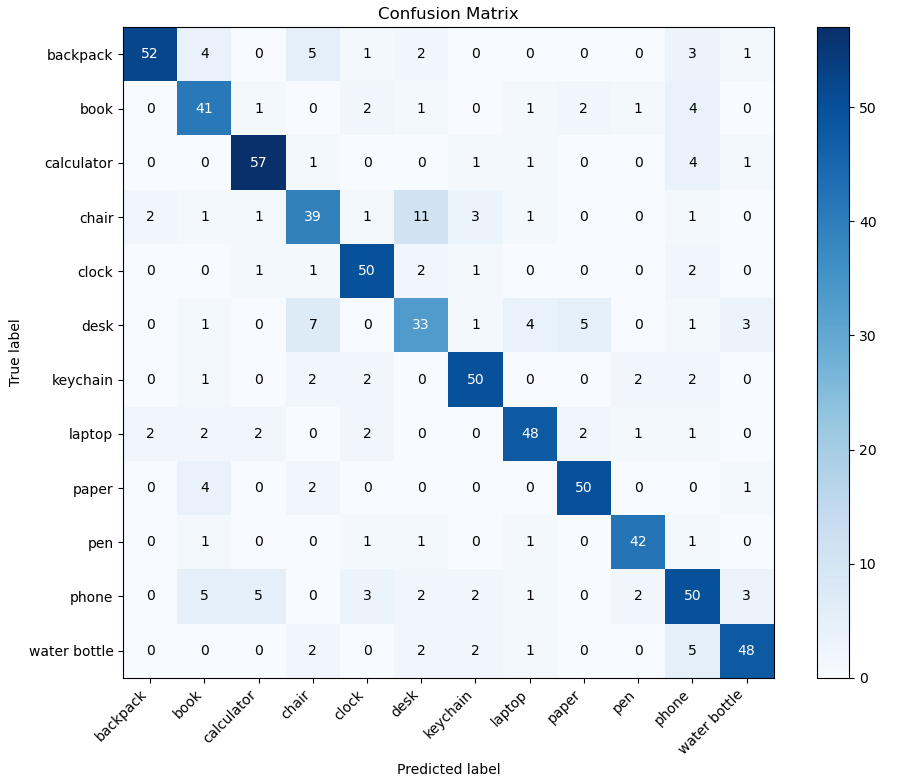
\includegraphics[width=0.9\textwidth]{figures/confusion.png}
    \caption{Confusion matrix for CNN classification model evaluated on the test set. Each row represents the true class, and each column represents the predicted class. The model shows high classification accuracy for most classes, especially calculator, pen, and paper, while confusion is observed between similar objects such as desk and chair, and phone and calculator.}
    \label{fig:confusion}
\end{figure}

\subsection{Results Analysis}

Table 1 already shows that our CNN model achieves an overall test accuracy of 78.43\% versus only 7.56\% for the random guessing baseline an improvement of 
70.87 percentage points. A more detailed analysis of how the models performance on different classes differs is as the following:

\subsection{Analysis of Per-Class Performance}
\paragraph{Highest Gains}  
The largest improvements over random chance occur on:
\begin{itemize}
  \item \textbf{Clock:} +84.21 pts (87.72\% vs.\ 3.51\%)
  \item \textbf{Pen:}   +82.98 pts (89.36\% vs.\ 6.38\%)
  \item \textbf{Calculator:} +78.46 pts (87.69\% vs.\ 9.23\%)
\end{itemize}

\paragraph{Lower Gains}  
Smaller improvements are seen on:
\begin{itemize}
  \item \textbf{Desk:} +52.73 pts (60.00\% vs.\ 7.27\%)
  \item \textbf{Chair:} +58.33 pts (65.00\% vs.\ 6.67\%)
  \item \textbf{Phone:} +61.64 pts (68.49\% vs.\ 6.85\%)
\end{itemize}

\paragraph{Effect of Test Set Distribution}
Analyzing the per-class performance in relation to the number of images in each class shows that there is no direct correlation between class size and classification accuracy.
\begin{itemize}
  \item \emph{Phone}, the most common class (73 images), achieved a modest accuracy of 68.49\%, which is lower than average.
  \item \emph{Pen}, the least represented class (47 images), achieved the highest accuracy of 89.36\%.
\end{itemize}
This suggests that class frequency on its own does not determine model performance. It can potentially be explained that having clearer, more distinctive visual features (e.g., pens, clocks, calculators)
is what really influence CNN accuracy to be higher instead of just the number of examples in each class.

\paragraph{Consistently Strong Classes}
Several mid-sized classes performed particularly well:
\begin{itemize}
  \item \textbf{Clock (57 images)} and \textbf{Calculator (65 images)} both achieved nearly 88\% accuracy.
  \item \textbf{Paper (57 images)} and \textbf{Keychain (59 images)} also scored above 84\%.
\end{itemize}
These results further confirms the idea that the CNN benefits from learning distinct shapes and textures, as many of these objects have well-defined and distinct appearances.

\paragraph{Weaker Classes and Ambiguity}
\begin{itemize}
  \item \textbf{Desk (55 images):} 60.00\%
  \item \textbf{Chair (60 images):} 65.00\%
\end{itemize}
Classes with lower accuracy like \emph{Desk} and \emph{Chair} suggest that visual ambiguity may hinder classification, even when test counts are moderate. The given images of desks or chairs may have appeared in a wider range of angles, lighting conditions compared to other classes. Furthermore, the many different designs and appearances that they might come in could have also made it harder for the model to generalize. Additionally, this low accuracy may be attributed to pictures in the \emph{Chair} and \emph{Desk} class also containing objects of the other classes, as pictures with desks in them often also have chairs and pictures with chairs in them often have desks. This same confusion likely occurred with other classes as well, specifically misclassifying the desk class frequently because the desk images may contain laptops, papers, or water bottles.

\subsection{Summary}
Regardless of a few underperforming classes, our model has significantly outperformed the random guessing baseline by 70.87 percentage points overall, reaching a 78.43\% accuracy, with every class achieving more than a 50-point gain. 
This demonstrates that our CNN model is effective at classifying images into the 12 object classes. 





%% TODO: write about what you conclude. This is not meant to be a summary section but more of a takeaways/future work section.
%% Must contain:
%% - Any concrete takeaways or conclusions from your experiments/results/project
%%
%% You can also discuss limitations here if you want.
%%
\section{Conclusions}
This project successfully demonstrated the effectiveness of convolutional neural networks in multi-class image classification tasks, even with a small dataset. The results demonstrate:

\begin{itemize}
\item \textbf{Effectiveness of Data Augmentation:} Using data augmentation techniques significantly improved our model's generalization ability, preventing overfitting and improving performance, which is important when working with limited data.

\item \textbf{Regularization Strategies:} Using dropout layers, batch normalization, and weight decay effectively combated overfitting issues, demonstrating the importance of regularization techniques in deep learning models.

\item \textbf{Hyperparameter Optimization:} Fine tuning of hyperparameters, including learning rate, batch size, and model complexity, was essential in maximizing model accuracy.

\item \textbf{Class Distinguishability vs. Frequency:} Model performance was impacted greatly by the clarity and distinctiveness of class features rather than class frequency, emphasizing that dataset quality and diversity in features is just as if not more important than having a large number of images per class.

\end{itemize}

\paragraph{Future Work:}
Several steps could be taken to further improve the performance and robustness of our classification model:

\begin{itemize}
\item \textbf{Better Labeling:} The worst performing class, \emph{Desk}, would benefit from multi-label classification,  allowing images to have multiple labels if they contain several objects (e.g., desk + chair + laptop).

\item \textbf{Transfer Learning:} Leveraging pre-trained models through transfer learning might significantly boost accuracy and be particularly beneficial for classes with ambiguous features.

\item \textbf{Ensemble Methods:} Implementing an ensemble of CNN architectures or using techniques such as bagging or boosting could further increase the accuracy and generalization capabilities of the classifier.

\end{itemize}

In conclusion, this project illustrates the usefulness of convolutional neural networks in image classification tasks, emphasizing the importance of effective data preprocessing, strategic model design, and sufficient regularization to achieve reliable, accurate results.

%%%%

\bibliography{refs}
\bibliographystyle{plain}

\begin{itemize}
\item \textbf Course Slides

\end{itemize}


\end{document} % end tag of the document
